\documentclass[main.tex]{subfiles}
%\usepackage[T1]{fontenc}
%\usepackage{ae,aecompl}


%%%%% AUTHORS - PLACE YOUR OWN PACKAGES HERE %%%%%

% Only include extra packages if you really need them. Common packages are:
%\usepackage{graphicx}	% Including figure files
%\usepackage{amsmath}	% Advanced maths commands
%\usepackage{amssymb}	% Extra maths symbols
%\usepackage{lipsum}
%\usepackage{lmodern}
%\usepackage{tcolorbox}

%\newcommand\levelone[1]{{\color{red}\bf}}
%\newcommand\leveltwo[1]{{\color{blue}\bf}}
%\newcommand\levelthree[1]{{\color{green}\bf}}
\begin{document}

\chapter{Life emerges...}

\par \nar For a long while, there was only darkness.  Well, mostly darkness.  Light is to the Universe what germs are to the world.  In a nutshell, that stuff is pretty much \textit{everywhere}.  You're basically constantly being bombarded by individual particles of light, called photons,$^{\textcolor{red}{\ref{boxchap1:photons}},\textcolor{red}{\ref{boxchap1:photons}}}$ when on Earth.  This is still the case even when your eyes are telling you it is black and there is no light.  So remember, just because you can't see light does not mean it isn't there.  Just like germs.

%\footnote{Photons are particles of light.  They travel freely through vacuum at a speed of about 299792458 meters per second or 299792 kilometers per second or, if you prefer, 671000000 miles per hour; basically photons travel an unfathomable distance each and every second.  Photons are defined according to their energy or, equivalently, wavelength or frequency.  The spectrum of energies characterizing photons is called the electromagnetic (EM) spectrum.  Photons are produced in the cores of stars, eventually working their way up to escape from the surface.  These photons, often mostly from the visible portion of the EM spectrum, are transparent to the Earth's atmosphere.  They are detected by our eyes, revealing a wonderfully brilliant and colorful night sky on Earth.}  

%\section{Hello World} \label{hello}
\section{A Star is Born} \label{born}

\par \nar On a very fateful day, everything changed.  Cosmic Dawn emerges with a roar.  The veil of darkness is lifted.  An especially massive Giant Molecular Cloud is in the final stages of contracting, becoming more and more dense as time goes on.  The internal pressure from within, provided by the random motions of her constituent atoms and molecules, guides the hand of gravity to re-shape her into a critical new state.  Over-dense knots and filaments begin to form within her belly.  The knots continue to coalesce, becoming ever hotter and denser.  Finally, new life emerges.  Deep within one such dense knot, the massive protostar \rmmaia is born, weighing in at a whopping 5 M$_{\odot}$ , or 5 times the mass of the Sun.

\par \nar With her birth, comes Dawn.  Protostars spew out light in the form of photons at a thunderous pace; enough to make the radiation emitted by an unfathomable mound of radioactive waste completely negligible by comparison.  Seven siblings, all due to be born within the narrow window of a few million years. Their Mother, \rmpleione, a particularly compelling Giant Molecular Cloud, now begins her journey through Motherhood.  But it's not yet over; she's still in the process of yielding to gravity's nurturing might, slowly contracting and compressing, forming over-dense filaments and birthing new stars, buried deep within her belly.  

%LEVEL ONE:
%\begin{tcolorbox}[sharp corners, colback=red!30, colframe=red!80!blue, title=Photons]
%\lipsum[2]
%\par \textcolor{red} {Photons are particles of light.  They travel freely through vacuum at a speed of about 299792458 meters per second or 299792 kilometers per second or, if you prefer, 671000000 miles per hour.  Basically, photons travel an unfathomable distance each and every second.  Photons are defined according to their energy or, equivalently, their wavelength or frequency.  The spectrum of energies characterizing photons is called the electromagnetic (EM) spectrum.  Photons are produced in the cores of stars, eventually working their way up to escape from the surface.  These photons, in particular those in the visible portion of the EM spectrum, are transparent to the Earth's atmosphere.  Photons from the visible portion of the EM spectrum are detectable by the human eye, revealing a wonderfully brilliant and colorful night sky on Earth.}
%\end{tcolorbox}

\par \Maia Hello to you, Mother!$^{\textcolor{red}{{\ref{boxchap1:st}},\textcolor{red}{\ref{boxchap1:st}}}}$

\par \Pleione Hello to you as well, my child.  My young new protostar!

\par \Maia Wow!  The Universe is so amazing and beautiful to behold.  Are all those twinkling things off in the distance other protostars, like me?

\par \Pleione Yes, my child.  Well, most are distant stars, not protostars.  Stars live long lives, and the protostellar phase$^{\textcolor{red}{{\ref{boxchap1:proto}},\textcolor{red}{\ref{boxchap1:proto}}}}$ does not last long; only a few million years or so.  So most of the far off stars you are looking at are much older than you.  The emitted light is what makes stars shine, taking many millions of years to travel from the center of the star to its surface.  This is because the individual particles of light bounce around inside the star, eventually arriving at the surface of the star after a prolonged random walk.  In the end, light escapes at a colossal rate as the photons leak through the star's surface, escaping into outer space.  And the light can travel very large distances before reaching you, the observer.  This is how you are able to see them in spite of those stars being so far away.  
%Light makes stars shine.  They can even appear to twinkle when very far away.
%\footnote{EXPLAIN TWINKLING!!!}


\par \Maia I see, stars live very long lives...  So, presumably, as I transition from a protostar to a real star, I too will have a very long life.  I'll take it!  

\par \Pleione How many stars do you see out there?

\par \Maia Uh... How \textit{many}?  I don't understand...

\par \Pleione Well, let's start at the beginning.  When it comes to counting, that is usually a good idea.

\par \Maia Counting?

\par \Pleione  Counting is a way to keep track of something.  For example, how much of something you have or can see, or how often something should happen.  In order to count, the first thing you will need is a numbering system.

%level one:
%\begin{tcolorbox}[sharp corners, colback=red!30, colframe=red!80!blue, title=Numbering Systems]
%\par \textcolor{red} {INSERT HISTORICAL CONTEXT/INFO ABOUT DEVELOPMENT OF NUMBERING SYSTEMS HERE.}
%\end{tcolorbox}

\par \Maia What is that?

\par \Pleione A numbering system uses symbols and rules to do the keeping track of things.  The symbols are called "numbers".  The rules decide how to use those symbols to do the counting.  The counting is done by performing operations, including addition, subtraction, multiplication, division, and so on.  For example, if you add two positive numbers together, you always get a bigger positive number.  If you add two negative numbers, you always get a smaller more negative number.  

\par \Maia I'm not sure I'm following you...

\par \Pleione Okay, well, before giving up on me, let me try to explain two very key concepts in any numbering system.  The first is "zero" (i.e., 0).  This number just means that you are without any of whatever it is that you are counting.  None.  The second is "one" (i.e., 1).  This number is pivotal to any numbering system, since it defines the unit of measure.  For example, I am your Mother.  I, and I alone, created you.  There is only one of me.  You are my child, and you are also unique since there is only one of you.  But, if I were to birth another star like you, then I would have more than one child.  In this case, I would have \textit{two} children.  This follows from defining the addition operator, such that $1 + 1 = 2$.  The operator acts to initiate some mathematical calculation, whether it be addition, subtraction, multiplication, division, etc.

\par \Maia I think I am following you now.  What if we go back to before I ever existed?  How many children did you have then?  Was it zero?

\par \Pleione That's right!

\par \Maia Okay.  So, there were zero children a long time ago.  Then there was one, or me.  And soon there will be two, if you give birth to another star.  Then... wait, what 's next?

\par \Pleione The next number in the sequence is three.  But, before we get there, let's take a moment to consider the concepts of addition and subtraction in a little more detail.

\par \Maia Fair enough.  What about them?

\par \Pleione These ideas are rather central to all of "mathematics", or using numbers to calculate or compute things.

%level one:
%\begin{tcolorbox}[sharp corners, colback=red!30, colframe=red!80!blue, title=History of Mathematics]
%\par \textcolor{red} {INSERT HISTORICAL PERSPECTIVE ON THE DEVELOPMENT OF MATH HERE.}
%\end{tcolorbox}

%\note{A.S.H.: I find the green boxes hard to read. Maybe we should tweak the colors a bit? Also,
%we should bear in mind that having a lot of color in the book (text boxes plus illustrations) could be costly when publishing!}
%\note{NWCL: Completely agree.  You can barely read the green text.  This is what I mean about the formatting - at some point we will have to make final decisions.  If you have any recommendations now though, let us start implementing them.}

\par \Maia You're losing me again...

\par \Pleione One way to calculate something is to add numbers together, as I have already shown you.  To summarize, I start by making one star.  I then make one more star.  Now I have two stars.  But each star is itself just one star.  So, here, we are adding one star together with another one star, and this gives us two stars.  So one plus one is equal to two, or 1 $+$ 1 $=$ 2.  We are adding stars together, and counting them as we go.

\par \Maia You're winning me back...  I think I'm following you...

\par \Pleione Now let's take it one step further.  If we have two stars, and we add one more star, how many stars do we have?

%level one:
%\begin{tcolorbox}[sharp corners, colback=red!30, colframe=red!80!blue, title=Mathematical Operations]
%\par \textcolor{red} {SHOW MATH, DEFINE THE MOST BASIC MATH RULES RELATED TO ZERO, ADDING, SUBTRACTING, ETC...  ADD HISTORICAL CONTEXT AS WELL.  DISCUSS OTHER NUMBERING SYSTEMS?  LOGARITHMS? } 
%\end{tcolorbox}
 
\par \Maia Uh... Give me a second to think about it... \textit{Three!?}

\par \Pleione That's right!  If we add another star, then 1 $+$ 1 $+$ 1 $=$ 3, and we would have three stars.  

\par \Maia Look at me, I am counting!  And adding!  I'm learning so much.  You drop the knowledge, and I pick up what you are putting down.  I'm even having fun!

\par \Pleione You most definitely are, my daughter.  Now, let me ask again:  How many stars do you see, twinkling off in the distance?

\par \nar \rmmaia turns her attention back to the distant stars.  

\par \Maia I see a LOT of stars!  In fact, I see so many I do not think I could count them all.  There are far too many tiny twinkling DotS\footnote{DotS is an acronym for "Dawn of the Stars".} to count!  Well, it would take you a VERY long time, I imagine.

\par \nar Something catches \rmmaia's curiosity, distracting her from counting.  She gasps in wonder.

\par \Maia Whoa, if you look closely at some of those distant stars, they appear to be arranged in interesting ways that make them resemble familiar or even just weird shapes.  Like, over there, I see \textit{three} stars that are bunched close together and form a straight line.

\par \Pleione Very good, \rmmaia.  You are counting!  That is Orion's Belt.  Good eye!  If you take a larger look at him, you will notice as well a torso, arms and legs.  

\par \Maia I think I see them... Wait what are arms and legs?  

\par \Pleione Orion the Hunter is in the form of a human.  I would describe humans as resembling deformed stars; they look similar, and come in various colors and sizes.  But they also come along with many protuberances, such as arms and legs, each with their own set of functions.   Orion is but one example of the many stories depicted in the night sky, assigned by that species.  Humans call these familiar stellar configurations ``constellations'', and they are meant to tell some important story about their history.  Humans have developed many stories to explain their origins, which they often refer to as "myths".

\par \Maia Have you ever seen one?

\par \Pleione One what?

\par \Maia A human.

\par \Pleione Oh!  Yes, once, quite some time back.  Awful, vile species.  Constantly shooting projectiles off of the surface of their tiny planet, littering outer space with their garbage.

\par \Maia Yuck.  That does sound gross.  
%Well, I thought the third leg should be shorter because it's supposed to be back a bit, and I thought that gives it a 3-dimensional feel.  What did \textit{you} think it is?

%\newpara \Pleione Uh... Hey! 
\par \Pleione Did you know that Orion the Hunter even has a bow to fire arrows at his enemies!?  If you look closely, you can see he is holding it in his left hand, and it forms a large arc in the sky.

\par \Maia I see it!... Wait... Enemies?  What kinds of enemies?

\par \Pleione Well, if you follow Orion's Belt from left to right, you will pretty quickly notice that it points to a very bright red star.  That is the star \rmaldebarran, the Eye of Taurus the Bull.$^{textcolor{red}{{\ref{boxchap1:ald}},\textcolor{red}{\ref{boxchap1:ald}}}}$  According to the myth, Orion the Hunter fought Taurus the Bull to save the Seven Sisters.  If you keep following that line, you will notice that it points to us.

\textcolor{cyan}{NL:  INSERT CAPTION EXPLAINING WHAT ORION WOULD LOOK LIKE FROM THE PLEIADES, RELATIVE TO EARTH.}

\par \Maia Wow, that sounds very dramatic.

\par \Pleione I suppose it must have been.

\section{The Demise of Pleione} \label{demise}

\par \nar \rmpleione~ was growing weary.  Her children shine bright,$^{\textcolor{blue}{{\ref{boxchap1:se}},\textcolor{red}{\ref{boxchap1:se}}}}$ emitting a wind of charged particles and photons.

\par \nar As the winds collide with the loving embrace of their Mother, they provide an outward pressure and she begins to disperse.$^{textcolor{blue}{{\ref{boxchap1:radpress}},\textcolor{blue}{\ref{boxchap1:radpress}}}}$  The birth of \rmmaia initiated the demise of her mother.  

\par \Maia Wait, Mother, where are you going?  

\par \nar \rmmaia, the second most massive of her soon-to-be-born siblings, wears a worried expression upon her face that begets deep concern for her fleeting Mother.  

%\Maia And why is the entire Universe spinning?  Ugh... I think I might be sick.

%\Mother My child, it is not the Universe that spins, but you.  All stars are born rotating, and you are no excpetion.  But fear not, you were also born with a magnetic field, and this will spin you down over the next several tens of millions of years.

%\Maia Oh, thank goodness.  For a second there, I was worried I would be rapidly rotating forever.  That's a relief.  But, wait, back to where you are going...? 

%\Maia Mother!  Mother!  Don't go!

\par \Pleione Oh, young one.  There is nothing to worry about.  I will be with you always, no matter what adventures befall you.  You are, after all, made from me.  
%Please, take me with you, with an open heart.

\par \Maia Okay, but this is all sounding suspiciously like a goodbye...

\par \Pleione All will be well, you will see.  You are only just now born and still contracting, as gravity continues to find its balance with the fires that now rage within your belly, spewing out energy in the form of light.  Soon, gravity will balance this outward source of pressure, and you will arrive at a stable size and mass that persists for many millions or even billions of years. Hydrostatic equilibrium awaits!$^{\textcolor{blue}{{\ref{boxchap1:he1}},\textcolor{blue}{\ref{boxchap1:he1}}}}$

\par \Maia Um... You're leaving me with a complicated technical term like "hydrostatic equilibrium"...?  What does that even mean?$^{\textcolor{green}{{\ref{boxchap1:he2}},\textcolor{green}{\ref{boxchap1:he2}}}}$

\par \Pleione It means that the energy produced within your belly must be strong enough to balance the inward force of gravity, to ensure stability.  You can think of it as a sign that you are healthy.  So long as you are in hydrostatic equilibrium, you never need to worry about your health.  Your radius and mass should remain more or less stable over very long timescales.$^{textcolor{green}{{\ref{boxchap1:radius}},\textcolor{green}{\ref{boxchap1:radius}}}}$ 

\par \Maia Okay, I will remember that one.

\par \Pleione Take care of your siblings for me...

%\newpara \Maia Uh... Okay...  Still kind of confused over here...
\par \nar \rmmaia and \rmpleione continue their conversation, \rmpleione doing her best to prepare her child and her yet-to-be-born siblings for their inevitable journey through the Galaxy.  \rmmaia learns a great deal about the cosmos, the births and deaths of stars, how star clusters form, and so on.

\section{Hello World} \label{hello}

\par \nar Shortly later, one of \rmmaia's siblings awakens.  \rmelectra~ emits a long, sleepy yawn.  The least massive of her siblings, \rmelectra weighs a mere 0.4 M$_{\odot}$.  \rmpleione turns her attention toward her newly born daughter.

\par \Pleione Behold!  Your sister awakens!

\par \Electra  Uh... Hi.

\par \Maia Oh, wow.  She is \textit{super} bright and, well, shiny.$^{textcolor{red}{10}}$  It hurts my eyes if I stare right at her... Wait, \textit{is} this hurting my eyes?  Like, could I go blind?$^{\textcolor{red}{{\ref{boxchap1:se}},\textcolor{red}{\ref{boxchap1:se}}},\textcolor{blue}{{\ref{boxchap1:bb}},\textcolor{blue}{\ref{boxchap1:bb}}},\textcolor{blue}{{\ref{boxchap1:color}},\textcolor{blue}{\ref{boxchap1:color}}},\textcolor{green}{{\ref{boxchap1:sbl}},\textcolor{green}{\ref{boxchap1:sbl}}}}$

\par \Pleione Only if you look directly at her.

\par \Maia But I already did that!

\par \Pleione Are you blind?

\par \Maia I don't think so.

\par \Pleione How can you be sure?

\par \Maia Well, I can see you wincing, for one thing.  You are looking at me as if I just got in to a fight with a much more massive star and lost.

\par \Pleione Uh... I'm sure you'll be fine. Plus, it could have been worse.  It could have been a black hole!  They pack a far greater punch than any star, let me tell you.

\par \Maia Wait, what is a ``black hole''?$^{\textcolor{red}{{\ref{boxchap1:bhs}},\textcolor{red}{\ref{boxchap1:bhs}}}}$  They sound terrifying.

%level two
%\begin{tcolorbox}[sharp corners, colback=blue!30, colframe=blue!80!blue, title=Light From Accreting Black Holes]
%\par \textcolor{blue} {EXPLAIN HOW HIGH-ENERGY RADIATION BEING EMITTED WHEN BLACK HOLES ACCRETE MATTER!!!}
%\end{tcolorbox}


\par \Pleione Let's save that one for another day, child.  You've already had quite an eventful day.

\par \nar \rmpleione's gas tendrils, swirling and coalescing around her birthing children, gently touching and massaging their young faces, continue to dissipate, faster and faster with the birth of each new star.

\par \nar \rmelectra~ interrupts them suddenly, belching loudly.  Plasma is ejected from her surface.  It emanates from above the equator, around which a gaseous disk has now formed.  

\par \Maia I see you have a disk encircling you, \rmelectra.  I think I can even see a few planets forming!  They are still in the process of being birthed, but it looks like so far you will be hosting at least four satellites.  So far I think I can see three planets forming, and one moon!

\par \nar \rmelectra~ belches another time, louder than before.

\par \Electra I am eagerly waiting to meet them.  I hope this whole planet-birthing thing won't take too much longer.

%\begin{tcolorbox}[sharp corners, colback=blue!30, colframe=blue!80!blue, title=How do Planets Form?]
%\par \textcolor{blue} {Discuss planet formation theories briefly, and an associated timescale for planet formation, related to the survival time of typical protoplanetary disks.}
%\end{tcolorbox}

\par \nar Her daughters now nearly all born and slowly coming to life, \rmpleione's time has arrived. \rmpleione~ bestows one last kiss upon her daughters, before floating off and dispersing in to the infinite vacuum of outer space.

\par \Electra I am excited to be here, and to be part of the team. ...I feel as though I just missed something important though.  Please do fill me in.  What did I miss?  ...Wait, what are those two whispering about?

\par \nar Both \rmmaia~ and \rmelectra~ turn their gaze toward \rmtaygete~ and \rmalcyone~, who together form a compact binary star system.$^{\textcolor{blue}{{\ref{boxchap1:bs}},\textcolor{blue}{\ref{boxchap1:bs}}}}$

\par \nar Bound together by gravity, the sisters orbit their mutual center of mass in harmony, much like planets orbit stars.  The two sisters are in fact twins, each with a total mass of 2.1 M$_{\odot}$.  Needless to say, they were close, both in terms of their physical properties and the distance separating their centers of mass.  \rmtaygete~ and \rmalcyone~ quietly conferred about the topic at hand, namely which of the two of them is the brightest.

%MUST DO:
%PIPE:  CAN WE MAKE A MAP OF THE GALAXY WITH THE LOCATION OF THE PLEIADES INDICATED, AND EACH STAR'S TRAJECTORY THROUGH THE GALAXY?  FOR CHAPTER ONE?

\par \Taygete I think it goes without saying that I am brighter than you are.

\par \Alcyone Dream on!  I outshine you for sure.

\par \Taygete Alright, tough stuff.  Want to know how I know that I am brighter than you are?

\par \Alcyone Sure.  Amuse me.

\par \Taygete I'm definitely fatter than you are, and bigger.  Both contribute to making me brighter, relative to \textit{you}.  At least, I'm pretty sure that is how it works...$^{\textcolor{blue}{16}}$


%\begin{tcolorbox}[sharp corners, colback=green!30, colframe=green!80!blue, title=Stefan-Boltzmann Law]
%\par \textcolor{green} {}
%\end{tcolorbox}

\par \Alcyone Oh shut up...  You are neither fatter nor bigger than I am.  You \textit{are} way more delusional then I am though.  I'll give you that.

\par \nar Magnetic fields are responsible for ejecting plasma from the surfaces of stars, often in the form of filaments that follow the magnetic field lines.  In general, the faster the star rotates, the stronger is its magnetic field.  \rmtaygete~ and \rmalcyone~ use this effect to strengthen their magnetic fields temporarily, by increasing their rate of rotation.  Long filaments of plasma wave out from their respective surfaces, not unlike arms reaching outward.  They begin flailing at each other violently, intent on a fight.  But the gas tendrils lie outside of each other's grasp, unable to reach with even the longest tendril of plasma either can muster.  A sisters' quarrel unrealized.  Their efforts futile, they quickly give up.  

\par \nar \rmtaygete~ and \rmalcyone~ are in fact two members of a triplet.$^{\textcolor{red}{17}}$  \rmcelaeno, the third component of the triplet, lies much farther away than the other two.  This, combined with the fact that she is a more massive star weighing in at 4.0 M$_{\odot}$, makes \rmcelaeno a little bit different from her twin sisters.  She is often ridiculed by her fellow twins because of it.

\par \nar The triplets' current configuration, hierarchical and dynamically stable,$^{\textcolor{red}{18}}$ is nothing short of fate; binding them to each other practically indefinitely.

\par \Maia Well, I think you are almost certainly identical twins.  I cannot see any real difference between you.  I mean, look at $\rmcelaeno$ over there; she's blue, whereas the two of you are clearly more of a yellow color.  She's also \textit{much} fatter and bigger than the two of you combined.  

\par \Celaeno Alright, I see your point.

\par \Taygete Agreed.  \rmalcyone, I'd extend a hand in offer of peace, but I don't have one.

\par \nar \rmtaygete once again churns her inner dynamo, brightening in response.  Tendrils of hot plasma shoot outward from her surface, mimicking arms and hands that wave at her sister.$^{\textcolor{red}{19}}$

\par \nar Meanwhile, \rmcelaeno~ was inspecting her midsection meticulously.  Yep, fatter.  Unsure as to whether or not this was a good thing, \rmcelaeno~ wore a pensive expression, clearly trying to work it out in her head.  Before she could sort it all out, \rmtaygete~ interrupted her train of thought...

\par \Taygete Hey Celaeno!  I have a joke for you!

\par \Celaeno Okay!  I would love to hear it.

\par \Taygete. Okay, here goes:  How many blue stars does it take to screw in a lightbulb?

\par \Celaeno I don't know... Hmmm... One?

\par \Taygete Yep!  You got it!  Now let's see if you can get this one:  How many yellow stars does it take to screw in a lightbulb?

\par \Celaeno Um... One?

\par \Taygete Nope!  Wrong!  The answer is:  Nobody knows, since no yellow star has ever tried.  Yellow stars are smart enough to realize that they outshine any lightbulb by an unfathomable amount.   Hence, plugging in a light bulb is a waste of time for any star. For this reason, no yellow star has ever even bothered to try.

\par \Celaeno Oh, I get it then...  Blue stars are dumber than yellow stars.  Ha!...  Wait...

\par \nar \rmcelaeno looks down at herself, recalling that, unlike her yellow sisters, she is blue.

\par \Celaeno Oh...  Ouch.

\par \Alcyone Good one, sister!  She never even saw the punch line coming.  No surprise there, she's just a dumb blue star after all.

\par \Taygete. Exactly!

\par \Celaeno. Wow, you guys are awfully mean.

\par \nar \rmcelaeno~ started to wonder what life would be like alone with her twin sisters.  She was distracted when she noticed a dense whisp of \rmpleione passing between her and her twin sisters.  

\par \Celaeno What's that?

\par \Maia The fleeting remains of our Mother, I am afraid.

\par \Electra That's \textit{Mom}?!

\par \Maia Well, what's left of her.

\par \nar The siblings continued to accrete mass in the form of gas from what remained of their Mother, \rmpleione.  They each grew and grew, until eventually they reached hydrostatic equilibrium, arriving at a long-lived stable configuration.$^{\textcolor{blue}{20}}$  

\par \nar This marked the end of their growth, and ultimately the end of the protostellar phase of their lives, along with the becoming a bona fide star.  In the end, the outward pressure produced from within due to the thermonuclear reactions brewing in their bellies had grown sufficiently strong to balance the inward pull of gravity.  Hydrostatic equilibrium achieved!  With this balance in place, the siblings would endure most of their lives in this stable configuration, slowly fusing the lowest mass nucleon (hydrogen) into the next best thing (helium).

\par \nar \rmsterope~ came to life suddenly, announcing her appearance with a high-pitched scream.  With a mass of 2.93 M$_{\odot}$,\rmsterope appears most similar to \rmtaygete and \rmalcyone relative to her other siblings.

\par \Sterope AAAAAAAHHHHHHhhhh!!!!!  What the...?  Where am I?  What am I?  When...?  You get the idea.

\par \Maia It's okay, sister.  You are one of us.  We are stars born of the gas and dust of our Mother, a particularly glamorous Giant Molecular Cloud, if I do say so.  She has left us now, but not without first bestowing her deepest gift upon us all, along with all of her love.

\par \Sterope  Uh... You are all my sisters?  We are a family?

\par \Maia Yes!

\par \Sterope  In that case, there remains a slim chance that the rest of this conversation will proceed without me feeling the need to scream again.

\par \Maia Progress!

\par \Sterope Uh, yeah, right.  Progress.  Let's get down to the important stuff.  Who are all you strangers?  You are my sisters, that much I have gathered.  But what else?  Wait, who am \textit{I}?  More importantly, \textit{what} am I...?  I'm starting to feel another scream coming on...

\par \Maia Relax, young one.  You're in good company here.  Familiar company.  \textit{Familial} company, even. We are your siblings and we are stars.  Thus and therefore, you too are a star.  In fact, you are a star that is host to two satellites, called planets. 

%n mass, size and compositiu, n to Jupiter and Saturn.
\par \Sterope Holy cow!  You're right.  I have two planets.  Uh....hello there!  How, er, are you?  Do you have names?

\par \Alphab I'm okay!  Happy to be here.  My name is \rmalpha.  My sibling over there, orbiting you further out than I do, is \rmbeta.

\par \Sterope \rmalpha and \rmbeta!  What wonderful names.  I am \rmsterope, and I look forward to getting to know you both better.

\par \Betab Thank you, Mother.  We feel the same way. ...Wait, can we call you Mother?

\par \nar \rmsterope shrugged rather nonchalantly.

\par \Sterope Sure.   Why not?   Okay, getting back to my questions...  What is a star?  And does it have anything to do with why I am feeling so bloated?

\par \Alcyone I wasn't going to say anything, \rmsterope, but you do look a little red in the face.  Is everything okay over there?  Wait, you asked a good question.  What the heck is a star, anyways?$^{\textcolor{red}{3}}$

\par \Maia We are born of our Mother.  Plain and simple.  We formed out of the gas and dust she left behind, after gravity coalesced us into the beautiful burning spheres of hydrogen you see before you.  Inside, we home a nuclear furnace that generates energy and emits light.  Our insides are so hot, that hydrogen is converted in to helium, releasing energy in the form of light or what are called photons.  The hydrogen is our food!  Outside, gravity pushes inward, but it cannot surpass the outward push provided by our internal metabolisms.  Protostars will continue to contract to a denser state with a hotter core, until a critical balance is achieved, called hydrostratic equilibrium.  This will also get rid of the reddish hue you currently find yourself with, \rmsterope.

%\leveltwo
%\begin{tcolorbox}[sharp corners, colback=blue!30, colframe=blue!80!blue, title=Blackbody]
%\par \textcolor{blue} {A blackbody is an idealized object that absorbs all the incident radiation that falls on it at all frequencies.  Hence, incident visible light will be absorbed and not reflected, causing the surface of the object to appear black.  An ideal blackbody in thermal equilibrium adheres to two important properties.  First, it is an ideal emitter.  This means that, at every frequency, it emits as much or more thermal radiation compared to any other body at the same temperature.  Second, it is a diffuse emitter.  This means that the radiation is emitted isotropically or, equivalently, the emitted radiation is the same in all directions, when the radiation is measured per unit area perpendicular to a specified direction.}
%EXPLAIN BLACKBODY.  EXPLAIN WIEN'S LAW AND THE RELATIONSHIP BETWEEN COLOR AND TEMPERATURE.}
%%\par \textcolor{blue} {\nar Discuss/define blackbodies, their properties, and how this relates to second law of thermodynamics.  Could include some math showing how to derive each limiting approximaiton (e.g., Rayleigh-Taylor Law, Wien's Law, etc.).}
%\end{tcolorbox}

\par \Sterope Well, that's a relief: the bloating is only temporary.

\par \Alcyone I think I am following what you are saying, at least so far.  What do we need to eat to keep ourselves going?  I mean, we must need energy?  Is this what those things you call photons provide to us?

\par \Maia Yes, exactly.  You have plenty of energy to keep you going for billions of years!  You're consuming the hydrogen you were born with; converting it in to helium right there in your belly.  It's a gift, just enjoy it.  The consequence of this act of consuming is that you shine very bright.  Photons are emitted every time four hydrogen atoms are consumed to produce helium, and they leak through your body and emanate from your surface.  Bright as a light!  The nuclear fuel already stored within you is sufficient to last millions, even billions, of years.  You'll be shinning practically forever!

\par \Celaeno Sounds to me like an awful lot of time to kill.

\begin{figure}
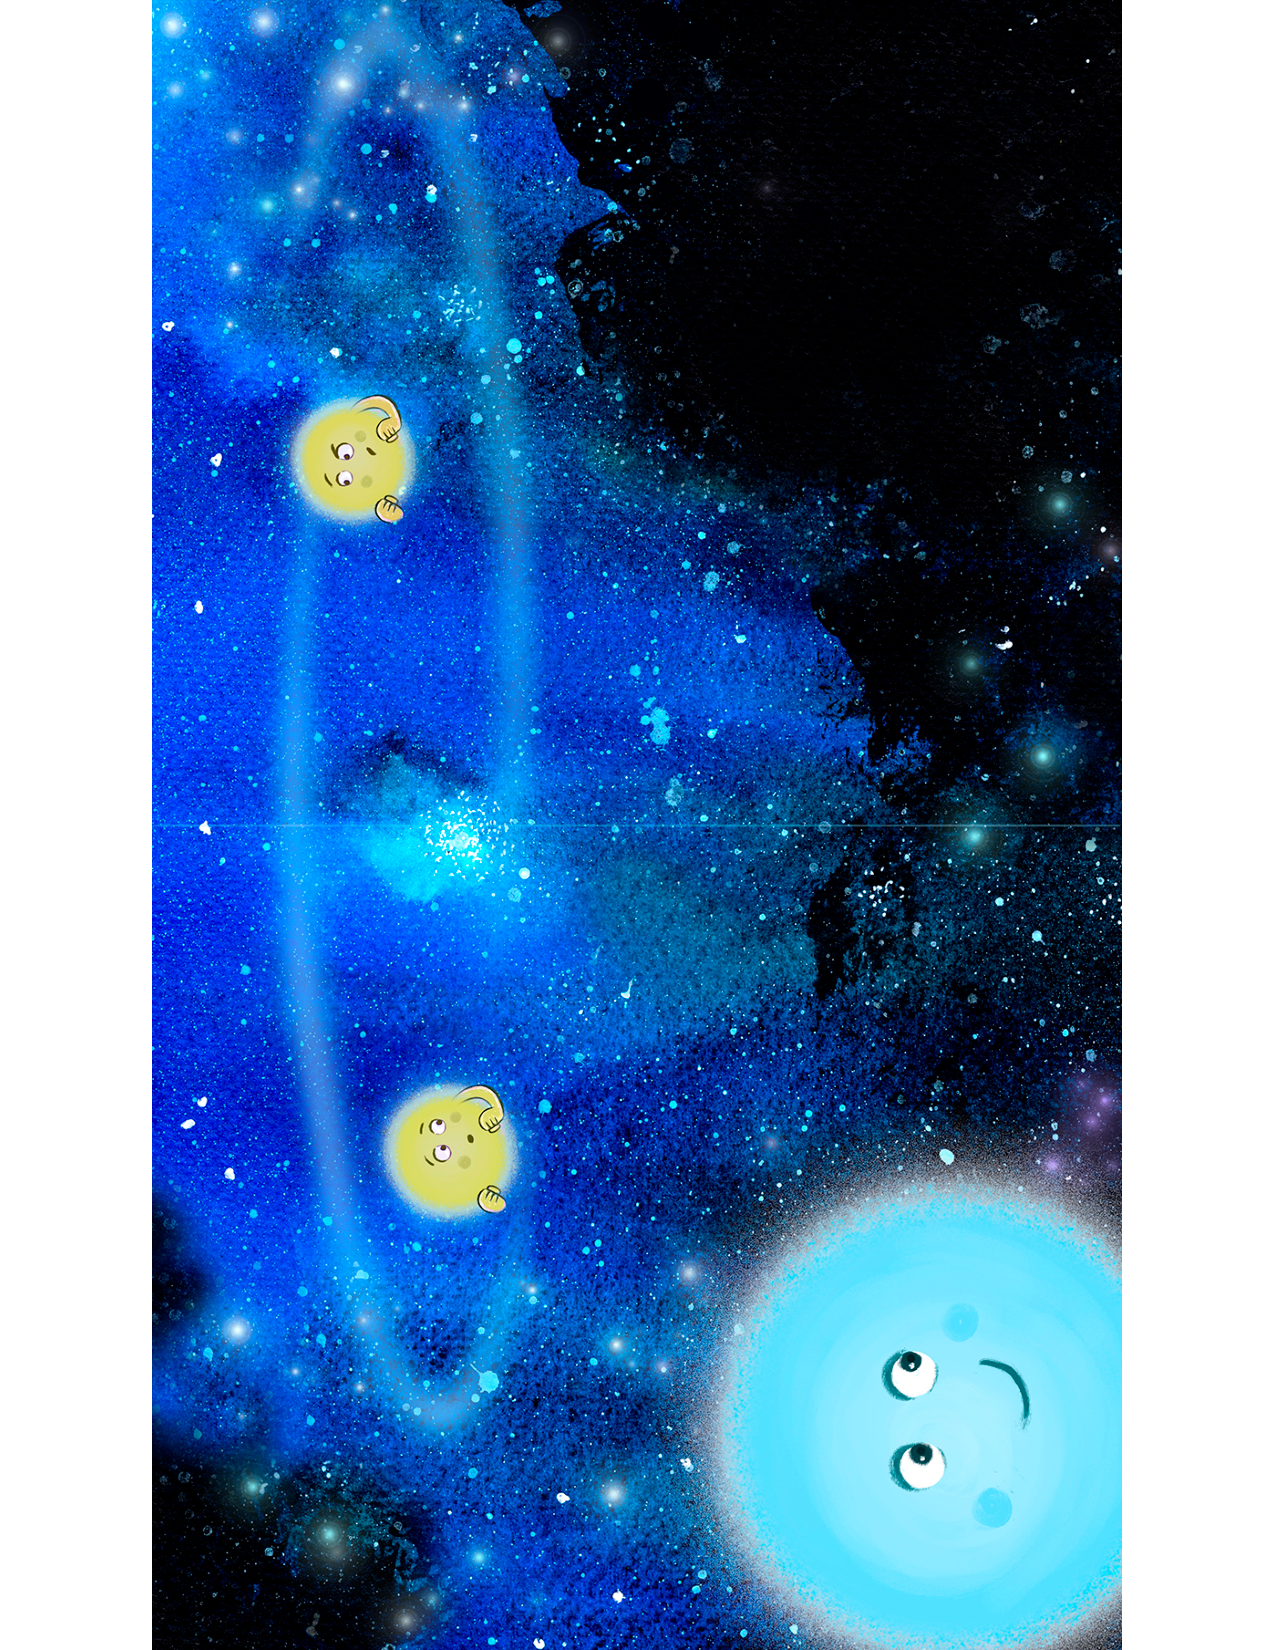
\includegraphics[width=\columnwidth,angle=270,origin=c]{ch1_2.pdf}
\caption{Taygete, Alcyone and Celaeno together.  Illustration by Andre Pipe Oliva.
\label{fig:fig2}}
\end{figure}

\par \Maia There will be plenty of adventures along the way to keep you distracted, I have no doubt.

\par \Sterope  Like what?  

\par \Maia Only time will tell.  But each star inevitably follows its own path through the Cosmos, and realizes its own fate.  We are individuals, after all.

\par \Sterope \rmmaia, how do you know so much?

\par \Maia Well, I don't really. I know what Mother told me.  I am the oldest of us, after all, and she explained as much as she could to me before dispersing.  

\par \Sterope I'm grateful for your efforts.  Mother dispersed so quickly, it must have been hard for her to convey a lot of detailed information to you before dispersing so completely.

\par \Maia It was.  She spoke really fast.

\par \Sterope And you remembered all of it?

\par \Maia Yep.  No problem!  

\par \Sterope Reeeeaaaaalllly, \rmmaia?  All of it?

\par \Maia \textit{Sigh}.  Fine!  Mother only told me a few things.  I don't want anybody to panic, so I'm trying to convey that Mother left me feeling confident, like we are more than capable of figuring it out for ourselves.  I'm only trying to help!  
%So there's a non-negligible chance that I'm making a lot of it up as I go along.  But \textit{most} of it is right, and straight from Mother.  At least... I'm pretty sure.  Take the filler with a grain of salt though.  

\par \Sterope Fair enough.  It sounds like you are doing your best.

\par \Maia I'm trying to motivate you, make you feel strong, loved and important!  ...Well, you get the idea.  With confidence, you can overcome any challenge that might befall you on your adventures.

\par \nar \rmmaia's shoulders slumped as she let out a prolonged sigh.

\par \Sterope It's okay, \rmmaia.  We love you too.

\par \nar \rmsterope~ flashes a warm smile at \rmmaia.  \rmmaia~ smiles back, relieved.  \rmalcyone~ belches loudly.

\par \Sterope \rmalcyone!

\par \Alcyone I'm sorry!  It was an accident.  I think it was that magnetic field thingy I have inside of me.$^{\textcolor{red}{21}}$  I'm learning that spontaneous emissions are, unfortunately, inevitable.  Way out of \textit{my} control, at least.

\par \nar Synchronized to the microsecond, \rmmaia~ and \rmsterope~ both roll their eyes.

\par \Maia Just do your best to keep your spontaneous emissions to yourself.

\par \Alcyone Will do. 

\par \Electra Uh...\rmmaia, I definitely don't mean to startle you, but some freaky, ominous stuff is going on right behind you.

\par \Maia Your goal there was to \textit{avoid} startling me?

\par \Electra Yep.  How'd I do?

\par \Maia Not very well at all.  I'm currently terrified of what might be lurking behind me.  Okay, I am turning around now...

\par \nar \rmmaia~ turns to see gas and dust had coalesced into a dense knot behind her.  She recognized right away the familiar dynamical dance of the gas choreographed by gravity; the final stages of the birth of yet another star, another sibling.

\par \Maia Oh, how wonderful!  We are witnessing the birth of our seventh sibling.  It would seem that Mother is not yet finished.

\par \nar \rmmerope~ came to life with a sudden jolt.  And the hiccups.  
%She is the second most massive of her siblings, weighing in at 4.5 M$_{\odot}$.

\par \Merope \textbf{Hiccup!}  Excuse me.  That whole being born thing was a little weird, and \textbf{Hiccup!} kind of uncomfortable.  It left with me extra gas in my belly, or \textbf{Hiccup!} something else that has given me the hiccups.  

\par \Alcyone It is the magnetic field inside of you!  It's nothing to be scared of though.  I'm just glad I'm not the only one spontaneously ejecting plasma!

\par \nar \rmmerope~ takes a minute to relax and compose herself.

\par \Merope Okay.  I'm feeling better now.  

\begin{figure}
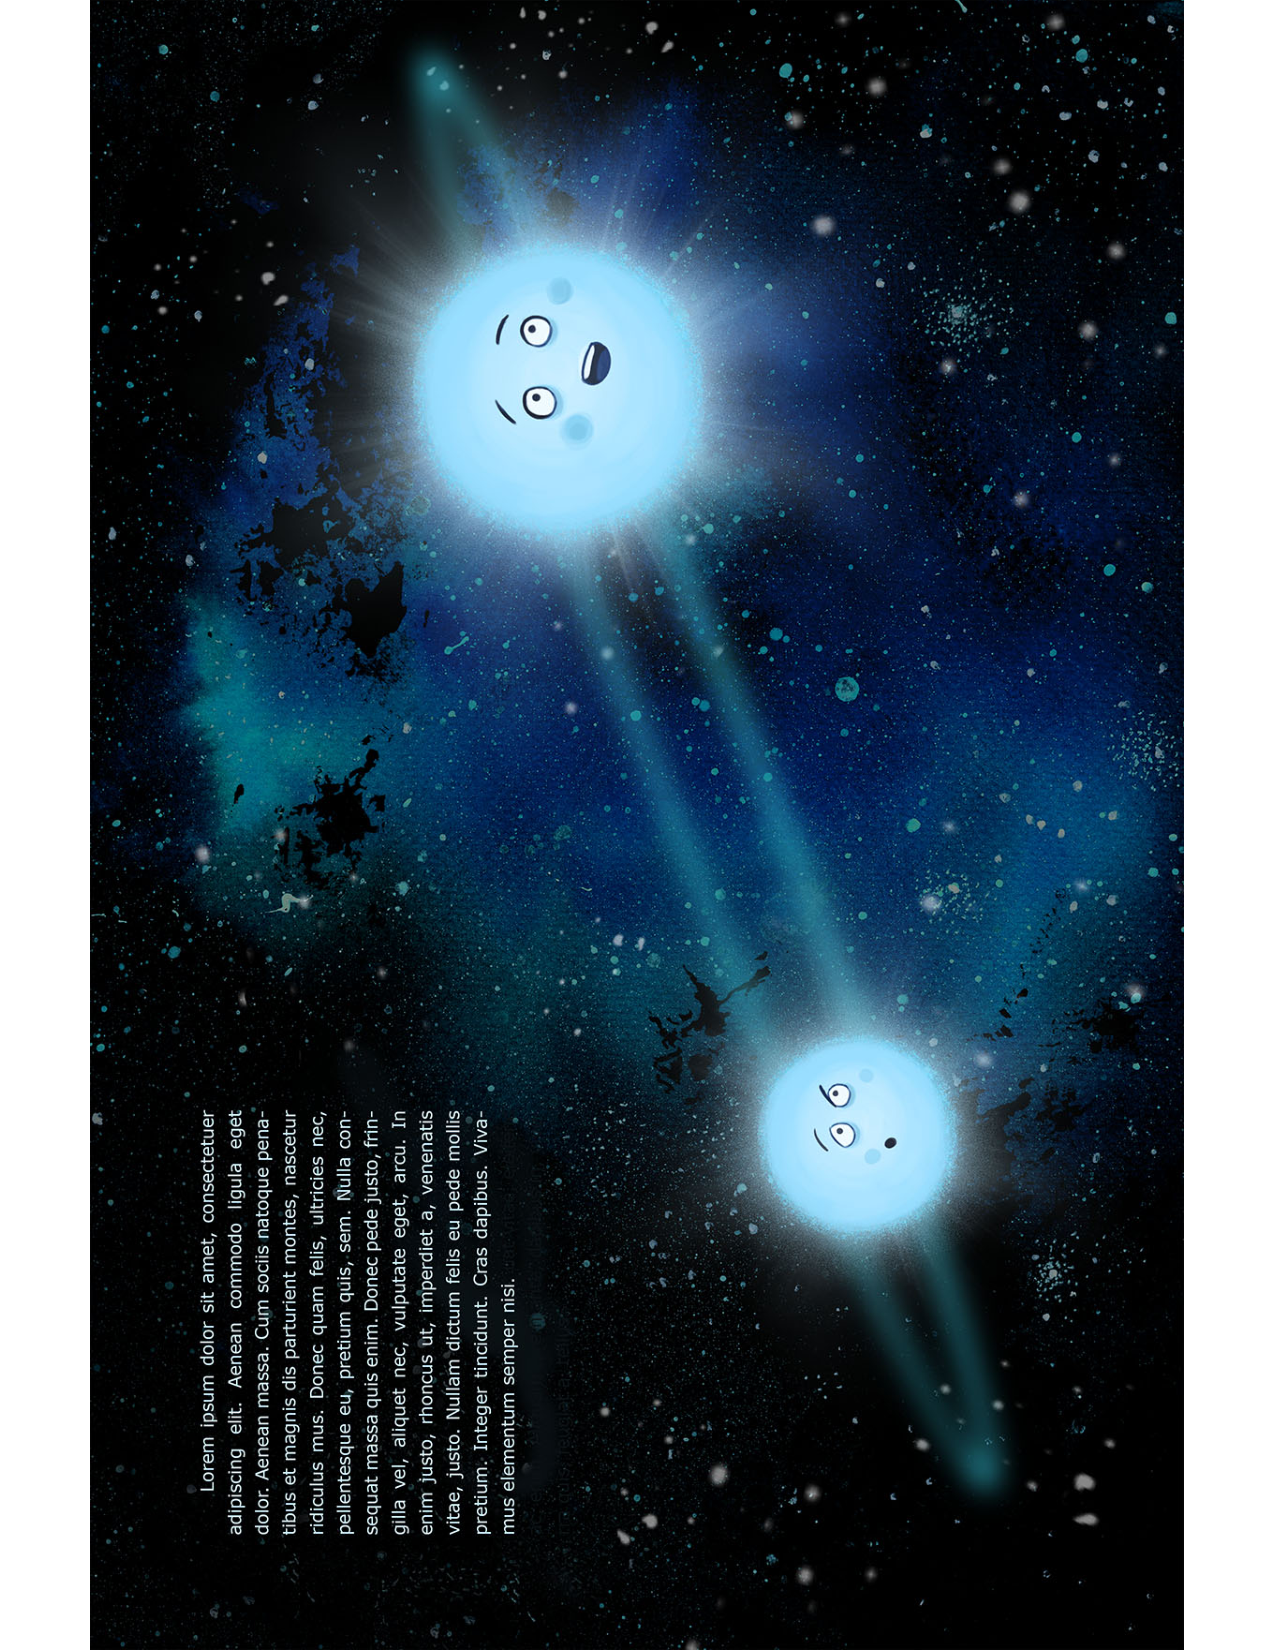
\includegraphics[width=\columnwidth,angle=270,origin=c]{ch1_1.pdf}
\caption{\rmmaia~ and \rmmerope, who together form a gravitationally bound binary star system.  Illustration by Andre Pipe Oliva.
\label{fig:fig1}}
\end{figure}

\par \Sterope Super!  I'll try to find solace in your comfort as I struggle to ignore the lingering stench of your quasi-belches...  Wait, who are you?

\par \Merope Oh right.  Introductions! I knew I was forgetting something.   Hi!  I'm \rmmerope!

\par \nar \rmmerope~ was the second most massive of her siblings, weighing in at 4.5 solar masses.  Gaseous emissions aside, her presence was hard to ignore amidst the seven sisters.  

\par \Maia It's wonderful to meet you, sister.  It would seem that you and I form a bound pair.  A binary star system!  How fortunate that gravity is an attractive force.  Our mutual gravitational attraction will keep us in this configuration practically forever.  Well, at least until one of us explodes or something.$^{\textcolor{blue}{22}}$

\par \Merope Wait, what!?  Who's exploding!?  Is it me!?  I don't want to explode!

\par \Maia Shhhh....  Relax, sister.  Nobody is exploding today.  
%, or tomorrow or any other day close enough to the present that we can count the number of days between now and then.  

\par \Merope Today!?  What about tomorrow?  

\par \Maia Nobody will be exploding tomorrow either.

\par \Merope And the day after that?

\par \Maia Nobody.

\par \Merope And the day after that?

\par \Maia Certainly not.

\par \Merope And the day after...?

\par \nar \rmmaia~ interjected before \rmmerope~ could finish.

\par \Maia Nobody will be exploding for a very long time, if ever.

\par \Merope Okay.  It doesn't seem immediately urgent, I guess. But we are \textit{definitely} circling back around to this exploding business at some point...

\par \nar Just then, a tiny voice made itself heard...

\par \Deltab I, for one, am very glad you will not be exploding, \rmmerope!

\par \nar The sisters turned in unison to behold the source of the voice, a small blue-green planet orbiting \rmmerope.

\par \Merope Oh my!  I am hosting a planet!  Uh... Hello there!  It's a pleasure to meet you.

\par \Maia Indeed, it is a pleasure for me as well!  We have one thing at least in common:  we both orbit \rmmerope!

\par \Deltab It's a pleasure to meet you both.  A great pleasure, in fact. Our mutual journey together through space and time will be nothing short of epic!

\begin{figure}
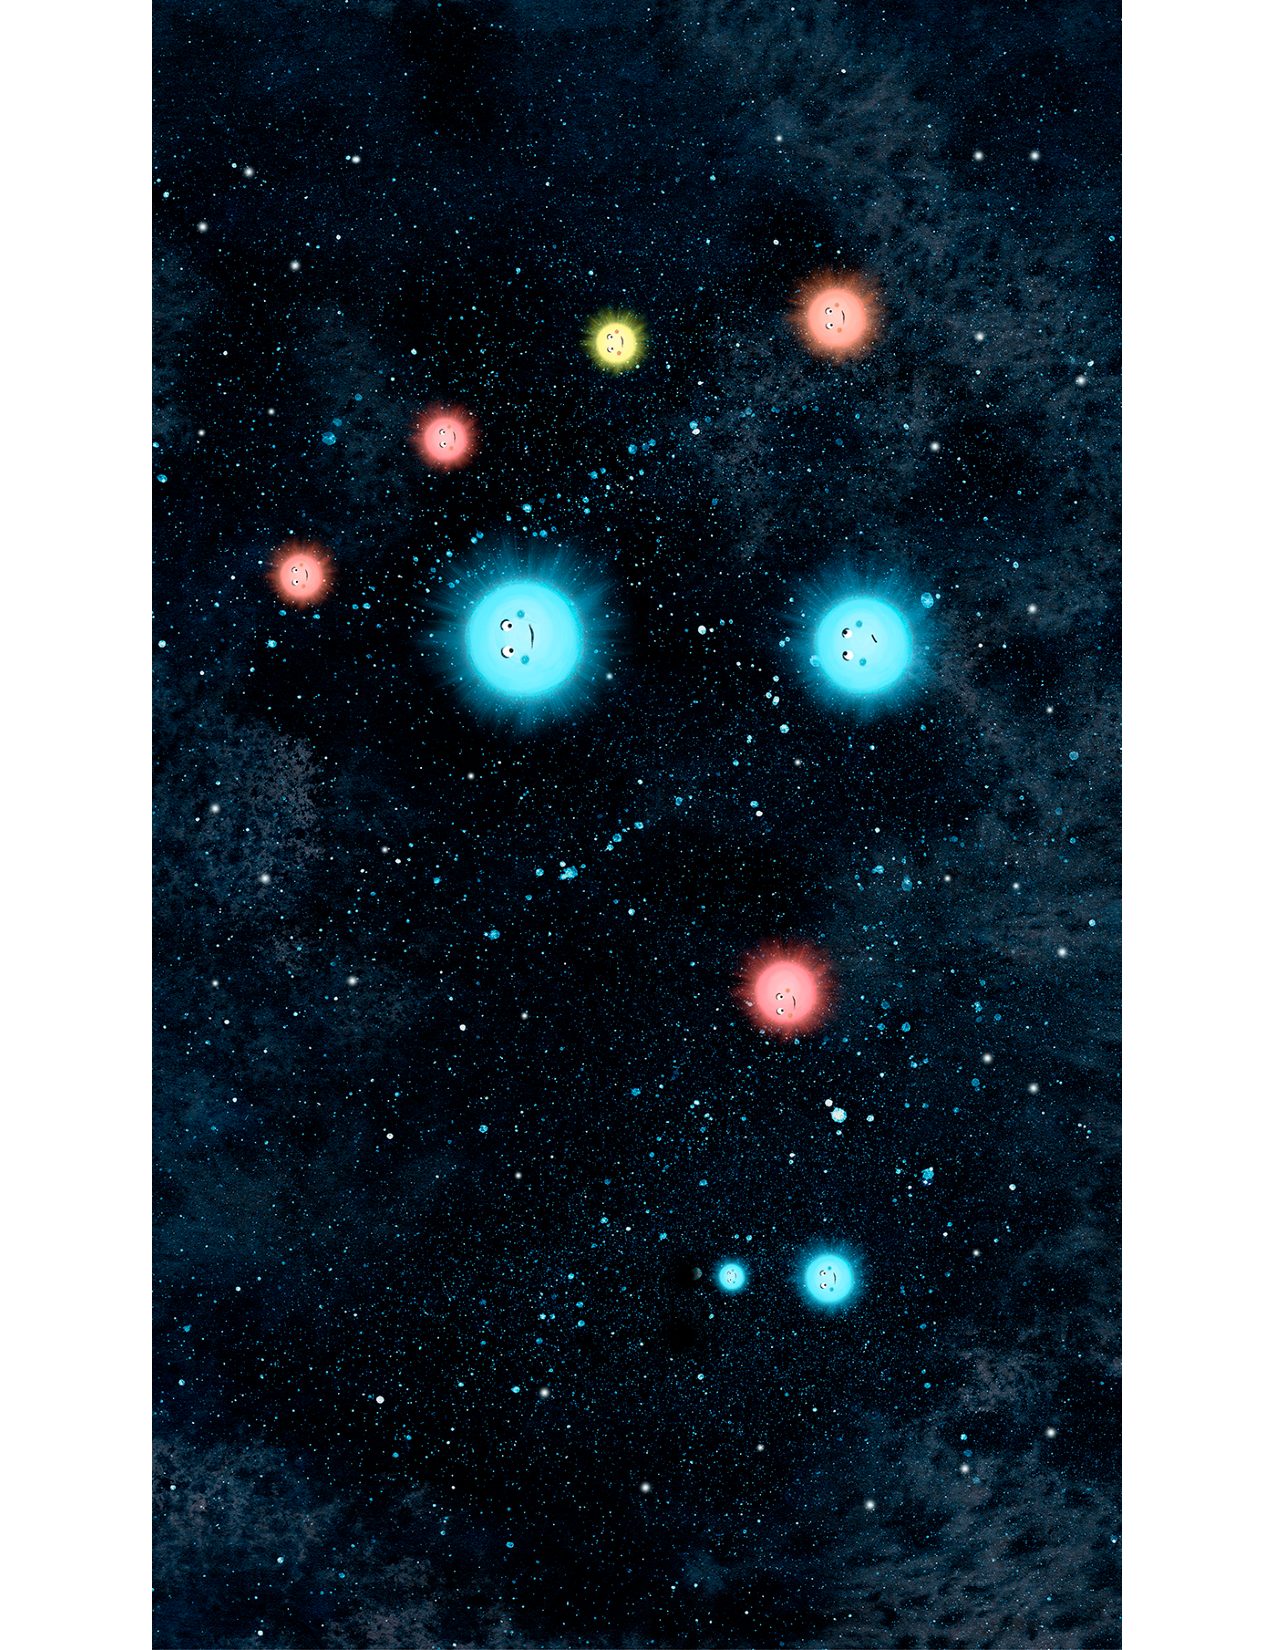
\includegraphics[width=\columnwidth,angle=270,origin=c]{ch1_3.pdf}
\caption{The seven sisters together, including Atlas and Lacedaemon to the left in the background.  Illustration by Andre Pipe Oliva.
\label{fig:fig3}}
\end{figure}

\begin{figure}
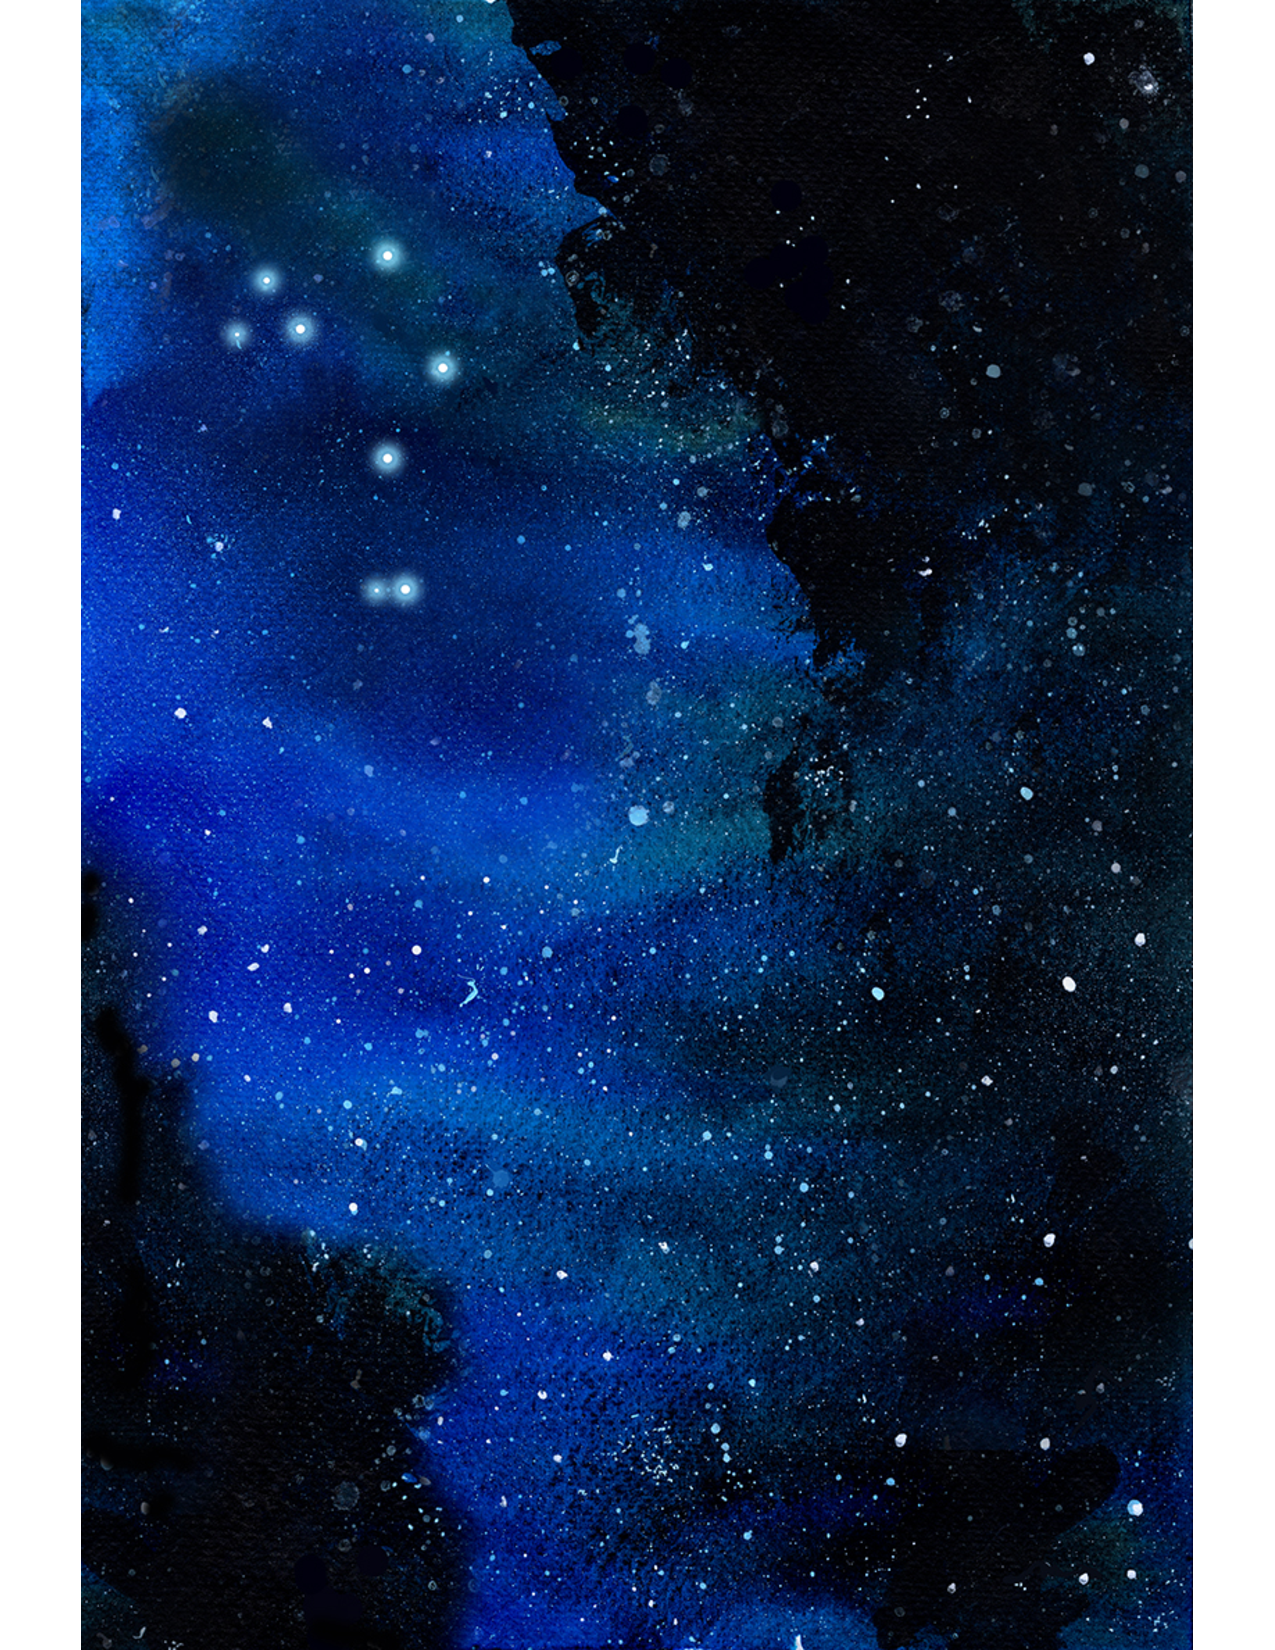
\includegraphics[width=\columnwidth,angle=270,origin=c]{ch1_4.pdf}
\caption{The Pleiades viewed from a distance, perhaps using a telescope on Earth.  Illustration by Andre Pipe Oliva.
\label{fig:fig4}}
\end{figure}


\par \Maia It will, I am sure.  I hate to change the subject, but at the moment it seems we have a family to become acquainted with.  I think that, together, we now form a young star cluster, our home.$^{\textcolor{blue}{23}}$

\par \nar \rmmaia~ turned to address her siblings.

%\textbf{THIS IS A GOOD PLACE TO INCLUDE ANY PLANETARY SYSEMS THAT ARE ALSO BEING BORN AROUND ANY STARS, IF ANYBODY WANTS TO INTRODUCE SUCH CHARACTERS.  NL:  I put several planets orbiting Electra... This was decided arbitrarily though, and we can change however we like moving forward.} 

%However, the most massive star clusters, may be the products of the mergers of several lower mass clusters.  The answer to this question is still an active area of research.} 

\par \Maia Greetings to you all!  I cannot express how happy I am on this day, the day of our mutual births.  The matter that forms our bodies comes from the same Mother, and to her we owe homage!  Our existence is blessed by her great sacrifice, having spent herself to birth us few.  Seven stellar siblings, and countless more familial satellites in the form of planets, moons, comets and even asteroids.$^{\textcolor{red}{24}}$  I see \rmelectra has a number of planets!
%with stable orbits about her center of mass!  

\par \Electra I'm as surprised as you are!  But I am eagerly looking forward to getting to know them better.

\begin{figure}
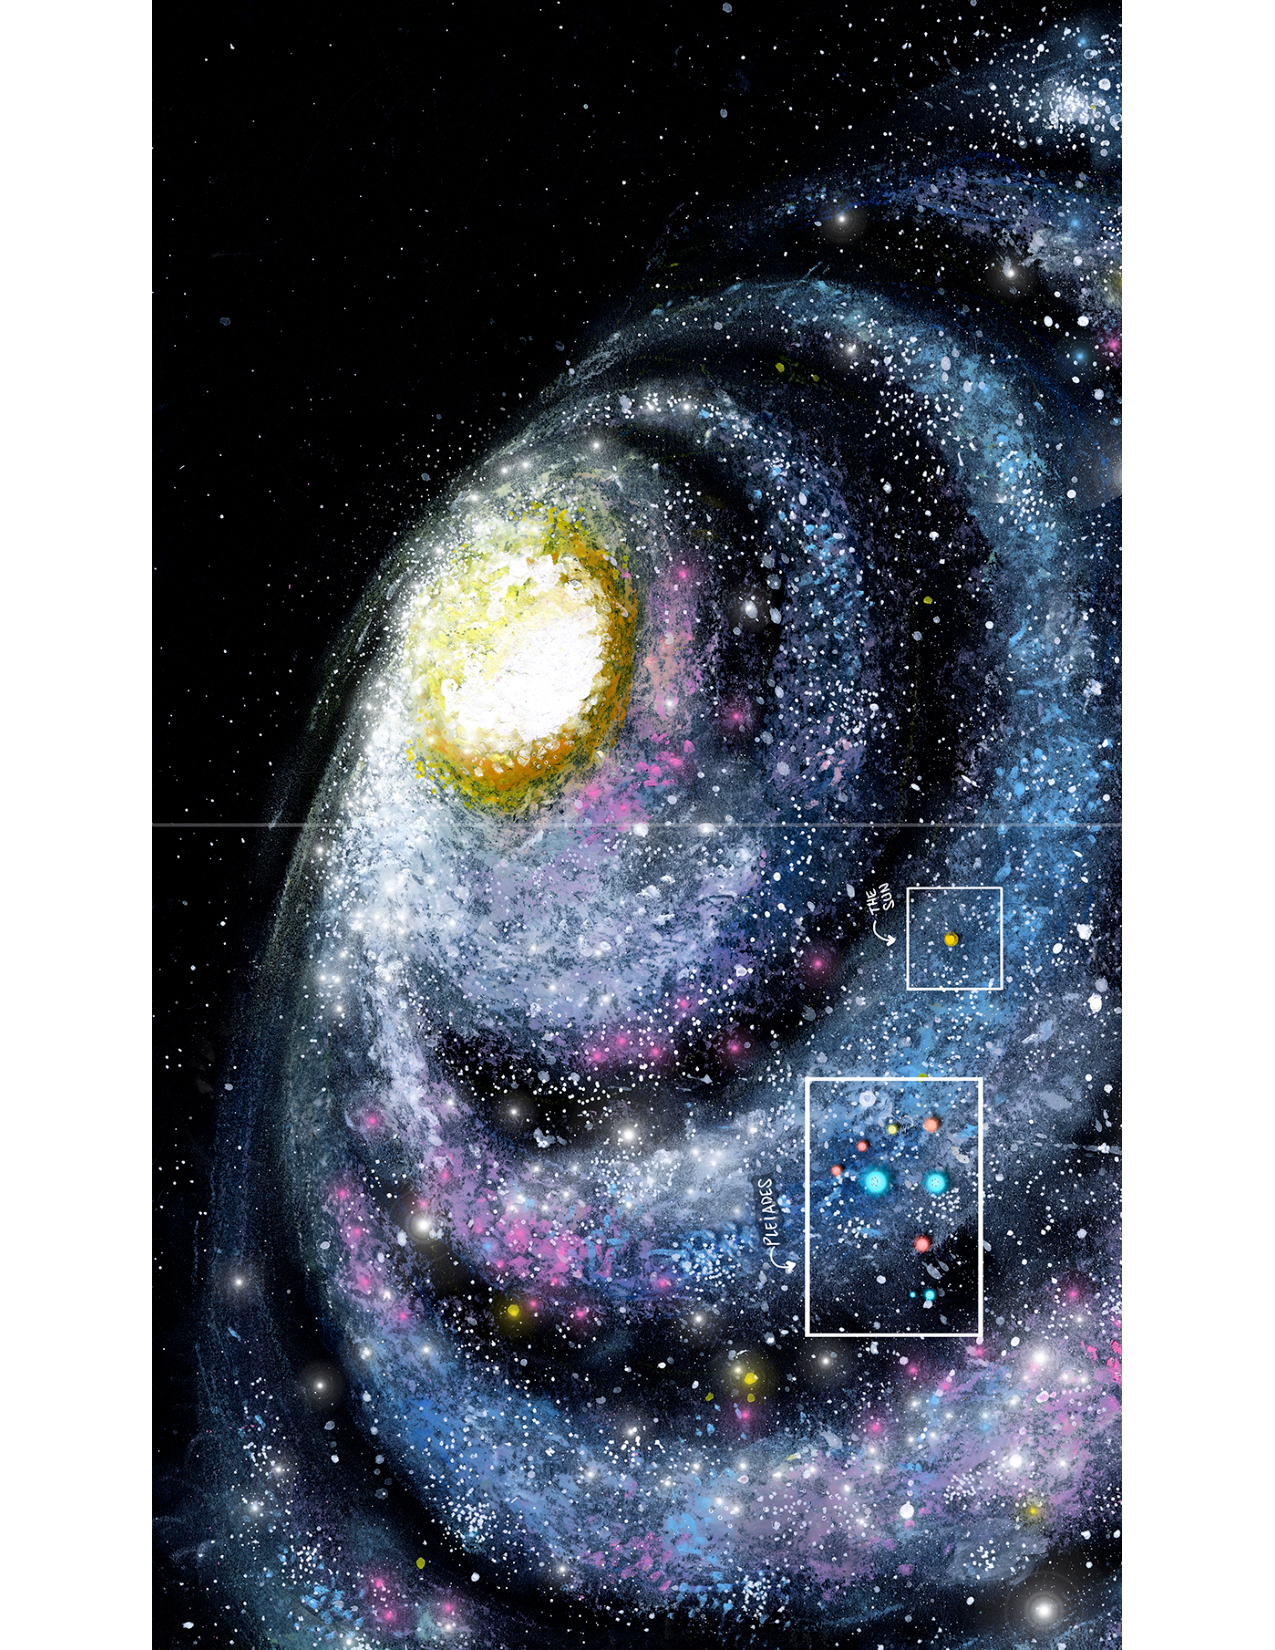
\includegraphics[width=\columnwidth,angle=270,origin=c]{ch1_5.pdf}
\caption{The location of the Pleiades star cluster in the Milky Way, relative to the location of the Sun.  Both the Pleiades and our Sun reside in the disk of our Galaxy, where star formation is still occurring.  Illustration by Andre Pipe Oliva.
\label{fig:fig5}}
\end{figure}

\par \Maia All born of the same stuff, in the same place, and at about the same time.  It is truly a time to celebrate.  But we are all weary of a prolonged dawn, and should now rest.  When we awake, we will celebrate properly!

\par \Merope  Count me in!  

\par \Electra A party sounds great. \textit{Yawn}. Just after I get a little shut eye.

\par \Sterope I could go for a nap. Then a party.  I'm in too.

\par \nar Meanwhile, \rmtaygete, \rmalcyone~ and \rmcelaeno~ had already fallen asleep, and were snoring loudly.  Seven siblings, all born within the narrow window of a million years.  The future looks bright for the Seven Sisters.

\section{Educational Material}

%LEVEL ONE:
\begin{tcolorbox}[sharp corners, colback=red!30, colframe=red!80!blue, title=Box \refstepcounter{educhap1}\label{boxchap1:ald}\ref{boxchap1:ald} -- Aldebaran]
\par \textcolor{black} {Aldebaran is the brightest star in the constellation Taurus.  At a mass of 1.7 M$_{\odot}$, Aldebaran is more evolved than the Sun, and is thus intrinsically brighter and redder.  Since it is in the process of ascending the giant branch of stellar evolution, it is preparing to fuse the hydrogen and helium in its core into more massive elements.  This phase of stellar evolution comes after the main-sequence phase, during which time hydrogen is being fused into helium in the stellar core, providing a net source of energy that eventually emerges from its surface in the form of photons.   As stars leave the main-sequence phase of evolution to ascend the giant branch, they begin to expand.  By the end of this phase of evolution, the radii of the stars can be inflated by several orders of magnitude relative to the main-sequence phase.  As the surface of the star is pushed farther and farther away from the core, where energy is being generated, its surface temperature drops.  As will explained in more detail as the story develops, this changes the star's color from yellow to red.  Hence, Aldebaran shines red, since its surface temperature exceeds 3,700 K, but is much lower than the 5770 K characteristic of the surface of our Sun.}
\end{tcolorbox}
%\lipsum[2]

\begin{tcolorbox}[sharp corners, colback=blue!30, colframe=blue!80!blue, title=Box \refstepcounter{educhap1}\label{boxchap1:photons}\ref{boxchap1:photons} -- Photons] 
\par \textcolor{black}{Photons are particles of light.  They travel freely through vacuum at a speed of about 299792458 meters per second or 299792 kilometers per second or, if you prefer, 671000000 miles per hour.  Basically, photons travel an unfathomable distance each and every second.  Photons are defined according to their energy or, equivalently, their wavelength or frequency.  The spectrum of energies characterizing photons is called the electromagnetic (EM) spectrum.  Photons are produced in the cores of stars, eventually working their way up to escape from the surface.  These photons, in particular those in the visible portion of the EM spectrum, are transparent to the Earth's atmosphere.  Photons from the visible portion of the EM spectrum are detectable by the human eye, revealing a wonderfully brilliant and colorful night sky on Earth.  But the EM spectrum is vast and the visible portion, namely the light humans can detect with their eyes, is only a small component of it.  So, as with germs, most of the photons landing on your skin cannot be seen with the naked eye.}
\end{tcolorbox}

\begin{tcolorbox}[sharp corners, colback=red!30, colframe=red!80!blue, title=Box \refstepcounter{educhap1}\label{boxchap1:st}\ref{boxchap1:st} -- Stellar Communication]
\par \textcolor{black} {Stars of course cannot speak.  But they can communicate with each other, even over very large distances.  They communicate by modulating their luminosities on short timescales, brightening and dimming, brightening and dimming, in whatever cadence properly communicates their intended message.  Humans are unable to speak, write or even read the language of the stars.  Throughout this book, all communications between stars will be expressed in English.} 
\end{tcolorbox}

\begin{tcolorbox}[sharp corners, colback=red!30, colframe=red!80!blue, title=Box \refstepcounter{educhap1}\label{boxchap1:prot}\ref{boxchap1:prot} -- From Protostar to Bona Fide Star]
\par \textcolor{black} {The transition from protostar to bona fide star can take several million years to complete.  During this time, the protostar is contracting, which it does by radiating away its excess energy via photons.  Upon losing this energy, the star will contract and become more compact.  This process continues until eventually the protostar becomes attains a stable state of equilibrium:  the inward force of gravity becomes balanced with the outward pressure provided by the energy leaking out of the star's core.  The star stops contracting and maintains a stable size or radius.  It is at this point that the protostar becomes a real star, entering the main-sequence phase of its evolution, during which time its energy is supplied by nuclear burning in the core, via the conversion of hydrogen into helium. \\
EXPLAIN P-P CHAIN?}
\end{tcolorbox}

%level one:
%\begin{tcolorbox}[sharp corners, colback=red!30, colframe=red!80!blue, title=Aldebaran$^4$]
%\par \textcolor{red} {Aldebaran is the brightest star in the constellation Taurus.  At a mass of 1.7 M$_{\odot}$, Aldebaran is more evolved than the Sun, and is thus intrinsically brighter and redder.  Since it is in the process of ascending the giant branch of stellar evolution, it is preparing to fuse the hydrogen and helium in its core into more massive elements.  This phase of stellar evolution comes after the main-sequence phase, during which time hydrogen is being fused into helium in the stellar core, providing a net source of energy that eventually emerges from its surface in the form of photons.   As stars leave the main-sequence phase of evolution to ascend the giant branch, they begin to expand.  By the end of this phase of evolution, the radii of the stars can be inflated by several orders of magnitude relative to the main-sequence phase.  As the surface of the star is pushed farther and farther away from the core, where energy is being generated, its surface temperature drops.  As will explained in more detail as the story develops, this changes the star's color from yellow to red.  Hence, Aldebaran shines red, since its surface temperature exceeds 3,700 K, but is much lower than the 5770 K characteristic of the surface of our Sun.}
%\end{tcolorbox}
%Describe what kind of star is Aldebaran...a red giant?  Describe the red giant phase of evolution.}

%\levelone
\begin{tcolorbox}[sharp corners, colback=blue!30, colframe=blue!80!blue, title=Box \refstepcounter{educhap1}\label{boxchap1:vt}\ref{boxchap1:vt} -- Virial Theorem]
\par \textcolor{black} {Over 10$^{38}$ photons are emitted every second.  Any tiny patch on the surface of a star is like the narrow entrance to a dark cave, with a swarm of bats flocking out from it.  Or germs, if you prefer.  In order to calculate the total energy emitted per second by the Sun, we can assume that every photon escaping from its surface has an energy of 12.86 Mev, corresponding to the highest energy photons produced at the end of the proton-proton-chain (thus our estimate here for the total number of photons should be regarded as a strict lower limit), which is the nuclear reaction process responsible for converting hydrogen in to helium.  Assuming 1 J $=$ 1.602 $\times$ 10$^{-13}$ MeV, we then calculate a solar luminosity of about 2.1 ${\times}$ 10$^{26}$ J s$^{-1}$.  This is very close to the total value of 3.828 $\times$ 10$^{26}$ J s$^{-1}$ computed for the luminosity of the Sun, calculated from integrated observations of the solar spectrum (REF). Finally, we note that [J s$^{-1}$] = [Watts].}  
\end{tcolorbox}

\begin{tcolorbox}[sharp corners, colback=green!30, colframe=green!80!blue, title=Box \refstepcounter{educhap1}\label{boxchap1:radpress}\ref{boxchap1:radpress} -- Radiation Pressure]
\par \textcolor{black} {Although photons do not have mass, they can still impart momentum by colliding with particles, including electrons, protons, atoms, molecules, and so on.  More stars means more photons, and hence more overall radiation pressure applied to dust particles, in this case the dust that constitutes the body of \rmpleione.  This accelerates the rate of dispersal of a surrounding cloud of gas and dust, since stars tend to be born near the centers of Giant Molecular Clouds where the gas densities are at their highest.  Hence, on average, radiation provides an outward source of pressure, moving away from the source of radiation responsible for producing the photons (e.g., nuclear burning in the cores of stars). \\
EXPLAIN MOMENTUM EXCHANGE USING IMPULSE ARGUMENTS, AND THAT LIGTH CARRIES MOMENTUM BUT NO MASS.}  %But how does this work?  DEFINE RADIATION PRESSURE.}
\end{tcolorbox}

%\levelone
\begin{tcolorbox}[sharp corners, colback=blue!30, colframe=blue!80!blue, title=Box \refstepcounter{educhap1}\label{boxchap1:he!}\ref{boxchap1:he1} -- Hydrostatic Equilibrium I]
\par \textcolor{black} {Hydrostatic equilibrium is what ultimately decides the size or radius of a star.  The term refers to the balance between the outward radiation pressure supplied by the energy released in the core via nuclear reactions producing photons (e.g., the proton-proton-chain, which is what burns hydrogen into helium) and the inward pull of gravity. \\
INCLUDE A DESCRIPTION OF CHANDRASEKHAR'S AND SPITZER'S CONTRIBUTIONS TO OUR UNDERSTANDING OF STELLAR STRUCTURE, AND EXPLAIN THE BASIC CONCEPT AGAIN USING THEIR VIRIAL THEOREM APPROACH.}
\end{tcolorbox}

\begin{tcolorbox}[sharp corners, colback=green!30, colframe=green!80!blue, title=Box \refstepcounter{educhap1}\label{boxchap1:he2}\ref{boxchap1:he2} -- Hdrostatic Equilibrium II]
\par \textcolor{black} {DERIVE THE EQUATIONS FOR HYDROSTATIC EQUILIBRIUM.}
\end{tcolorbox}

%level two:
\begin{tcolorbox}[sharp corners, colback=green!30, colframe=green!80!blue, title=Box \refstepcounter{educhap1}\label{boxchap1:radius}\ref{boxchap1:radius} -- What determines the radius of a star?]
\par \textcolor{black} {Stars out of hydrostatic equilibrium will either expand or contract.  If the pressure exceeds the gravity, then they expand.  If the gravity exceeds the pressure, then they contract.  This re-adjustment of the stellar radius is needed to set the right balance between pressure and gravity.  The radius of a star can only really be defined for stars in hydrostatic equilibrium, since the radius remain approximately constant in this state.  Conversely, for stars out of equilibrium, the radius is dynamically changing as the star re-adjusts itself to find a new stable balance between the outward pressure generated in the stellar core and the inward pull due to gravity. \\
But what supplies the outward source of pressure?  Sure, hydrogen is being burned into helium in the central cores of main-sequence stars, and this releases energy in the form of photons, but how exactly does this work?  INCLUDE DESCRIPTION OF THE P-P CHAIN.}
\end{tcolorbox}

%\levelone
\begin{tcolorbox}[sharp corners, colback=red!30, colframe=red!80!blue, title=Box \refstepcounter{educhap1}\label{boxchap1:se}\ref{boxchap1:se} -- Stellar Emission]
\par \textcolor{black} {Stars emit light spanning a wide range of energies.  The shielding effects of the Earth's atmosphere protect human eyes from very high-energy photons that would otherwise contribute to the degradation of the human eye.  From the surface of the Earth, we only see those photons within the visible portion of the electromagnetic spectrum.  But from space, our eyes would not be protected.  If stars' eyes are also sensitive to high-energy photons, then looking directly at other stars, especially very close ones, is anything but a good idea.}
\end{tcolorbox}

\begin{tcolorbox}[sharp corners, colback=blue!30, colframe=blue!80!blue, title=Box \refstepcounter{educhap1}\label{boxchap1:bb}\ref{boxchap1:bb} -- Blackbody]
\par \textcolor{black} {A blackbody is an idealized object that absorbs all the incident radiation that falls on it at all frequencies.  Hence, incident visible light will be absorbed and not reflected, causing the surface of the object to appear black.  An ideal blackbody in thermal equilibrium adheres to two important properties.  First, it is an ideal emitter.  This means that, at every frequency, it emits as much or more thermal radiation compared to any other body at the same temperature.  Second, it is a diffuse emitter.  This means that the radiation is emitted isotropically or, equivalently, the emitted radiation is the same in all directions, when the radiation is measured per unit area perpendicular to a specified direction.}
%EXPLAIN BLACKBODY.  EXPLAIN WIEN'S LAW AND THE RELATIONSHIP BETWEEN COLOR AND TEMPERATURE.}
%%\par \textcolor{blue} {\nar Discuss/define blackbodies, their properties, and how this relates to second law of thermodynamics.  Could include some math showing how to derive each limiting approximaiton (e.g., Rayleigh-Taylor Law, Wien's Law, etc.).}
\end{tcolorbox}

\begin{tcolorbox}[sharp corners, colback=blue!30, colframe=blue!80!blue, title=Box \refstepcounter{educhap1}\label{boxchap1:color}\ref{boxchap1:color} -- Why is a star observed to have a given color?]
\par \textcolor{black} {%EXPLAIN WIEN'S LAW, AND DISCUSS IN CONTEXT OF CONES IN HUMAN EYES. 
The color of a star, since star's are blackbodies, is largely decided by its surface temperature. Stars emit at all wavelengths since they are blackbodies, but their temperature decides the portion of the EM spectrum where most of the radiation is produced.  In general, the hotter the star, the more short wavelength light emits. The hottest ones are blue or blue-white, corresponding to the dominant emission being at shorter wavelengths. Cooler stars are red or red-brown, corresponding to longer wavelengths. 
But why do we not observe green or purple stars?  Human eyes have evolved to view predominantly yellow and green radiation, most likely because our sun emits radiation primarily in this wavelength regime.  A green star is mostly radiating in the center of the visible portion of the EM spectrum. The star should therefore appear white, due to a combination of the distribution of light that is emitted over the visible portion of the EM spectrum and the functionality of the human eyes, which have evolved to be more or less sensitive to certain wavelengths.  The human eye does not see purple stars for analogous reasons, namely because our eyes are more sensitive to blue light.  Hence, if stars are emitting similar amounts of purple and blue radiation, the human eye is sufficiently more sensitive to the blue contribution that this is what we tend to observe as the overall color of the star.}
%EXPLAIN BLACKBODY.  EXPLAIN WIEN'S LAW AND THE RELATIONSHIP BETWEEN COLOR AND TEMPERATURE.}
%%\par \textcolor{blue} {\nar Discuss/define blackbodies, their properties, and how this relates to second law of thermodynamics.  Could include some math showing how to derive each limiting approximaiton (e.g., Rayleigh-Taylor Law, Wien's Law, etc.).}
\end{tcolorbox}

\begin{tcolorbox}[sharp corners, colback=green!30, colframe=green!80!blue, title=Box \refstepcounter{educhap1}\label{boxchap1:sbl}\ref{boxchap1:sbl} -- Stefan-Boltzmann Law]
\par \textcolor{black} {DERIVE THE EQUATIONS FOR HYDROSTATIC EQUILIBRIUM.}
\end{tcolorbox}

%\levelone{
\begin{tcolorbox}[sharp corners, colback=red!30, colframe=red!80!blue, title=Box \refstepcounter{educhap1}\label{boxchap1:bhs}\ref{boxchap1:bhs} -- Black Holes]
\par \textcolor{black} {A good question.  We will learn a great deal about black holes over the course of this book.  For now, let us suffice it to say that many black holes are simply dead stars. Their progenitor stars ran out of nuclear fuel, which was providing the star with the outward pressure it needed to resist gravity's inward pull.  With no source of outward-directed pressure, gravity wins and the progenitor star collapses to form a new, much denser object.  If the progenitor star is sufficiently massive when it dies, it will collapse to form a black hole.  %From death, comes new life.  
Black holes are so dense that the strength of gravity forbids the escape of light from their interiors.  Thus, they are black, and do not emit light.  Until very recently and the invention of gravitational wave observatories, they have only been detectable by humans indirectly, via their gravitational influence on surrounding matter and stars.  But, with the introduction of gravitational wave measurements, we are now able to directly detect bound pairs of these objects just before they merge.  To date, this mainly applies to low-mass black holes, comparable in total mass to massive stars.  The origins of super-massive black holes, on the other hand, are thought to be much more complicated, and to this day remain shrouded in mystery.  This is because such massive black holes (with masses $\gtrsim$ 10$^5$ M$_{\odot}$) cannot have formed directly from stellar evolution and require additional physical processes to grow them to their currently observed masses.  This can occur by, for example, accreting matter from surrounding gas and stars.  But this is a story for another day.}
\end{tcolorbox}

%\leveltwo
\begin{tcolorbox}[sharp corners, colback=blue!30, colframe=blue!80!blue, title=Box \refstepcounter{educhap1}\label{boxchap1:bs}\ref{boxchap1:bs} -- Gravitationally Bound Pairs of Objects and Binary Star Systems]
\par \textcolor{black} {Two objects are said to be gravitationally bound if their total relative energy (i.e., the sum of their kinetic and potential energies) is negative.  In this case, the objects orbit their mutual center of mass, carving out circular or elliptic trajectories in a plane.  If both components are stars, such two-body systems are often referred to as binary stars.  The Earth is gravitationally bound to the Sun, as is the moon to the Earth.  Technically, the moon is also gravitationally bound to the Sun.  But gravity gets weaker with increasing distance, and the moon is close enough to the Earth and far enough away from the Sun that it orbits the former instead of the latter.}  
\end{tcolorbox}

%\leveltwo{
\begin{tcolorbox}[sharp corners, colback=blue!30, colframe=blue!80!blue, title=Box \refstepcounter{educhap1}\label{boxchap1:lum2 }\ref{boxchap1:lum2} -- Dependence of luminosity on Mass and Radius]
\par \textcolor{black} {The luminosity of a star increases steeply with both increasing mass and radius.  This is the case during the main-sequence phase of a star's lifetime, during which time stars are burning hydrogen into helium in their cores.  All stars, once finished with the protostellar phase, become main-sequence stars.  During later stages of stellar evolution, such as the red giant branch and asymptotic giant branch phases of evolution, the helium core sits at the center of the star, with hydrogen-burning occurring in the shell immediately outside the core.  Moving inward from the outer parts of the star and into the inner regions of the core, heavier and heavier elements are being produced, with each shell activating nuclear burning at a later time and corresponding to a different phase of stellar evolution.  Those shells forming the heaviest nuclei via nuclear burning are closest to the center of the star.  Moving outward from the center, each successive shell is burning lighter elements.  Hence, in very massive stars, hydrogen burning and helium formation occurs near the outer most shell, closest to the surface of the star.}
\end{tcolorbox}

%\levelone{
\begin{tcolorbox}[sharp corners, colback=red!30, colframe=red!80!blue, title=Box \refstepcounter{educhap1}\label{boxchap1:ds}\ref{boxchap1:ds} -- Dynamical Stability]
\par \textcolor{black}{Stable triple star systems are composed of three stars, and hence two orbits.  One of the orbits is very compact, and the other is very wide.  The outer orbit is so much wider than the inner orbit, that it is a good approximation for the outer tertiary to approximate the inner binary as a single object.  This is absolutely necessary to ensure the long-term dynamical stability of the triple.  If the inner pair becomes too wide, the gravity exerted by the outer object will pull the inner pair apart.  Chaos ensues.  This chaos can mediate the ejection of one or more stars from the triple, and even direct collisions.}  
\end{tcolorbox}

%\levelone{
\begin{tcolorbox}[sharp corners, colback=red!30, colframe=red!80!blue, title=Box \refstepcounter{educhap1}\label{boxchap1:oh}\ref{boxchap1:oh} -- Orbital Hierarchies]
\par \textcolor{black}{The easiest way to explain a "hierarchy" in a triplet is if two of the stars form a very compact binary, and the third star orbits at a very large distance from this compact pair.  Said another way, when it comes to a hierarchical triple star system, there are two orbits with almost opposing properties; the inner binary is compact, whereas the outer tertiary orbit is very wide.  In multi-planet systems, however, there can be multiple hierarchies.  For example, the Sun constitutes a significant fraction of the total mass of the Solar System, so all planets tend to primarily orbit its center of mass.  This is a hierarchy in mass - the planets are all much less massive than the Sun, so each planet's orbit can be approximated as an isolated two-body orbit between the planet and the Sun (i.e., ignoring the gravitational influence of the other planets is valid on short timescales). A second hierarchy in mass can appear if we now include moons, which orbit the centers of mass of the planets.}
\end{tcolorbox}

%\levelone{
\begin{tcolorbox}[sharp corners, colback=red!30, colframe=red!80!blue, title=Box \refstepcounter{educhap1}\label{boxchap1:mf}\ref{boxchap1:mf} -- Magnetic Fields and Dynamos]
\par \textcolor{black} {By making the inner core of a star rotate faster, an existing magnetic field can be amplified.   This can in turn trigger substantial chromospheric activity in the star, with filaments of hot plasma extending radially outward and coronal mass ejections bursting through its surface.}  
\end{tcolorbox}

%\levelone{
\begin{tcolorbox}[sharp corners, colback=blue!30, colframe=blue!80!blue, title=Box \refstepcounter{educhap1}\label{boxchap1:ss}\ref{boxchap1:ss} -- Steady State]
\par \textcolor{black} {The term ``steady-state'' implies a stable configuration, where all of the relevant forces or mechanisms have been balanced.  Here, it implies that the stars are maintaining an approximately constant mass and size, since they have reached a "steady-state", in this case hydrostatic equilibrium. \\
More generally, consider a spherically symmetric self-gravitating system of point particles.  The positions and velocities of every particle are described by a distribution function f($\vec{x}$,$\vec{v}$,t).  This distribution function can be evolved forward in time using a diffusion-based model, as is done in, for example, the classic Boltzmann equation or the radiative transfer equation.  According to Liouville's Theorem, if a system is in steady-state, then it must follow that:
\begin{equation}
\label{eqn:steadystate}
\frac{{\partial}f}{{\partial}t} = 0
\end{equation}
INCLUDE A DESCRIPTION OF DISTRIBUTION FUNCTIONS AND THE CRITERION FOR STEADY-STATE.} 
\end{tcolorbox}

%\levelone{
\begin{tcolorbox}[sharp corners, colback=red!30, colframe=red!80!blue, title=Box \refstepcounter{educhap1}\label{boxchap1:rec}\ref{boxchap1:rec} -- Reconnection of Magnetic Field Lines]
\par \textcolor{black} {Most main-sequence stars have magnetic fields that typically emanate from their poles; the younger the star, the more powerful the magnetic field.  When two or more magnetic field lines intersect, they ``reconnect'' to form new, disconnected field lines.  This ``reconnection'' is usually an energetic event, accompanied by a burst of high-energy photons (i.e., gamma rays and x-rays) and the ejection of plasma.}   
\end{tcolorbox}

%\levelone{
\begin{tcolorbox}[sharp corners, colback=blue!30, colframe=blue!80!blue, title=Box \refstepcounter{educhap1}\label{boxchap1:super }\ref{boxchap1:super} -- Supernovae and Stellar Lifetimes]
\par \textcolor{black} {The most massive stars end their lives with a dramatic explosion, called a supernova.  In one go, the explosion can liberate roughly as much energy as the Sun over its entire 10 billion year lifetime.  At their peak, supernovae shine 10$^{10}$ times brighter than the Sun.  There is a simple formula that allows us to calculate the expected lifetime of a main-sequence star, which is $\tau_{\rm MS} =$ 10(m/M$_{\odot}$)$^{-2.8}$ Gyr (REF? ADRIAN?).  Using this formula, for Merope, Maia, Calaeno, Sterope, Taygete, Alcyone and Elektra, we find MS lifetimes of, respectively, 0.1, 0.1, 0.2, 0.5, 1.3, 1.3, 130 Gyr.  As we will show later on, these lifetimes should exceed the timescale for the dispersal of the Pleiades open cluster. \\
INCLUDE A TABLE OF EACH OF THE SISTER'S OBSERVED PROPERTIES (SPECTRAL TYPE, MASS, COLOR, ETC.)}
\end{tcolorbox}

\begin{tcolorbox}[sharp corners, colback=blue!30, colframe=blue!80!blue, title=Box \refstepcounter{educhap1}\label{boxchap1:starclus}\ref{boxchap1:starclus} -- Star Clusters]
\par \textcolor{black} {As was the case for the Seven Sisters, most, if not all, stars are thought to be born in "clusters", gravitationally-bound and compact groupings of stars, ranging in numbers from a few tens to several million, with central densities in the range 10 M$_{\odot}$ pc$^{-3}$ - 10$^6$ M$_{\odot}$ pc$^{-3}$ or, equivalently, 10 - 10$^6$ stars per cubic parsec, where a parsec is defined as 1 parsec $=$ 3.086 $\times$ 10$^{16}$ meters.  These stars are all thought to form from the same Giant Molecular Cloud, as gravity shaped it into denser knots and filaments, creating the ideal environment for star formation.}  
\end{tcolorbox} 

%\levelone{
\begin{tcolorbox}[sharp corners, colback=red!30, colframe=red!80!blue, title=Box \refstepcounter{educhap1}\label{boxchap1:satellites}\ref{boxchap1:satellites} -- Satellites]
\par \textcolor{black} {The term satellite refers to any celestial body that is gravitationally bound to, but much less massive than, the massive object it orbits directly.  So planets, comets, asteroids, etc. are all satellites to stars.  Moons are satellites to planets.  Even stars can act as satellites, if they orbit a much more massive super-massive black hole.} 
\end{tcolorbox} 



\end{document}
